\section{Experimenting with Reaching (NoObs)}

\todo{structure this section and complete, some data from plots?}


\section{Increasing the Toy Task Complexity}
Complexity of tasks can be increased in two main ways:
\begin{enumerate}
  \item Introducing non-linearities to the environment to make a scene more challenging to traverse for an agent
  \item Increase the movement or the level of interaction of the task at hand
\end{enumerate}
I plan to do these mainly by introducing obstacles; which will guide me to understand what an agent needs to understand navigation. Secondly, I want to branch out to a grasping task, to increase the number of items of execution, to evaluate the capability of an agent to use its understanding to complete increasingly more complicated tasks.

\section{Reaching with an Obstacle}
To add onto the reaching task, I introduced an obstacle placing mechanism as well as randomly placing the target behind this obstacle, ensuring the agent doesn't learn where the target is by looking at just the obstacle. See Figure \ref{fig:reach-obs-random} for how this task looks and the check \todo{add appendix link, and code} for the backend wiring of these tasks.

\subsection{Creating the Task}

There are two versions of this task, I thought it might be interesting to randomise the object firstly dependently then independently on the obstacle. The `dependent' randomisation called \verb|ReachObs_Random| samples the obstacle, which in turn controls the spawn boundary of where the target can spawn in, meaning the target will always appear behind the obstacle albeit, edges of it can sometimes stick out. Conversely, the `independently' random version, called \verb|ReachObs_IndRandom|\todo{also add to appendix and link here}, this keeps the target spawn boundary fixed, meaning the target can be anywhere in the visible workspace, but it is not necessarily always covered by the obstacle. I can see that this potentially can be useful to keep the dataset a bit more diverse, and allow the wrist camera initially observe the target sometimes.\todo[color=red]{use this somewhere, or hint back to it, maybe even to say there was no difference}

\begin{figure}[htpb] % htpb allows all placement
  \centering
  \begin{subfigure}{0.3\linewidth}
    \centering
    \includegraphics[scale=0.3]{../fyp/assets/task-pics/reach-obs/random-front.png}
    \caption{Front}
  \end{subfigure}
  \hfill
  \begin{subfigure}{0.3\linewidth}
    \centering
    \includegraphics[scale=0.3]{../fyp/assets/task-pics/reach-obs/random-side.png}
    \caption{Side (Left)}
  \end{subfigure}
  \hfill
  \begin{subfigure}{0.3\linewidth}
    \centering
    \includegraphics[scale=0.3]{../fyp/assets/task-pics/reach-obs/random-top.png}
    \caption{Top}
  \end{subfigure}
  \vfill
  \begin{subfigure}{0.45\linewidth}
    \centering
    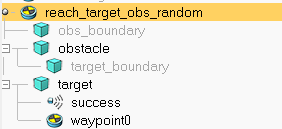
\includegraphics[scale=0.5]{assets/early-work/obs-random-scene-hierarchy.png}
    \caption{`ReachObs\_Random' Scene Hierarchy}
  \end{subfigure}
  \hfill
  \begin{subfigure}{0.45\linewidth}
    \centering
    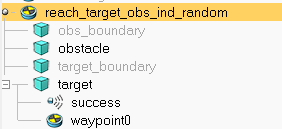
\includegraphics[scale=0.5]{assets/early-work/obs-ind-random-scene-hierarchy.png}
    \caption{`ReachObs\_IndRandom' Scene Hierarchy}
  \end{subfigure}
  \caption{Reaching Task with an Obstacle}\label{fig:reach-obs-random}
\end{figure}\todo[color=blue]{smaller?} 

\subsection{Experimenting with Views}\todo[color=red]{}

\subsubsection{Using same unchanged policy form ReachNoObs}
This is bad, the same will not work the demonstrations are not transferrable!!

\subsubsection{Understanding the Dataset}
Talk about how the data is loaded and created and managed for the network, talk about shuffling mechanisms and what I've found etc. talk about \verb|shuffle_obs_in_demo| and the other one.

\subsection{Improvements}



\subsubsection{Wrist Camera Alone isn't Enough}
As expected, this is where the single wrist camera started showing its shortcomings. 

\todo{add graph of going around the obstacle but not quite reaching the target (wrist)}
\todo{show this with other combinations of cameras, comment on if the l/r without wrist can learn to go around the obstacle easily? maybe not, generalisation might be hard with no wrist}

The agent would easily move around the obstacle, however, would struggle to make the last steps in touching the target. This is mostly due to the fact that the demonstrations (which are provided by RLBench) are not necessarily pointing the wrist of the robot and hence the camera mounted there to look towards the target. This means that the behavioural cloning agent learns to to the swaying motion around a large grey body, however, is not aware of the obstacle, or even understand the task is related to reaching for the obstacle and depends on its visual cues. 

From experiments I have realised that it learns to move around the obstacle easily, using simple behavioural cloning. However, getting the last nudge to actually reach the target is where it falls apart, especially in more realistic scenarios where the target is randomised behind the obstacle. For static placement behind the wall, the agent, expectedly is quite good. \todo{maybe explain or evidence this}

\subsubsection{Other Cameras}
Introducing the other cameras placed around in the environment, such as the \verb|left shoulder| or the \verb|right shoulder| cameras we can confirm that the wrist camera alone is not sufficient \todo{insert figure here with wrist vs others }, and the combination of wrist and other cameras are almost always the best as more coverage of the workspace guarantees less occlusions and more information the agent can work with to make decisions. It was clear that the wrist camera alone wasn't going to cut it unless it learnt to look towards the target.

\subsubsection{Multi Camera Mechanisms}
\todo{talk about `CamType' briefly}
\subsubsection{Policy Changes}
\todo{talk about the policy using differnt camera inputs to blend and make informed choices? maybe some plots here showing if it is better or not?}

\subsubsection{Implementing `Looking' into the Demonstrations}\todo{haven't done this yet}\label{ew-looking-at-target}
issues this is not easy might be working on this as a part of approach 2 later
Another solution might be to experiment with the demonstration system to make sure we are pointing the wrist camera (so, the hand of our robot) towards its target as a demonstration trajectory is calculated \todo{explain that this proved tricky and might not even be worth it}

If we can't implicitly encode the `looking' information through the demonstration that means we will have to inject this information into our agent some other way. Another way to make sure agent understands to look at the target is teaching it to actively seek out its target, either following previous works such as \todo{find some prior info tracking works add ref} where object priors are incorporated into the learning or with attention mechanisms that figure out what is important in a task without prior object information \todo{maybe reference this later}.  

\todo{this is important for plan2 later, as that would depend on such a mechanism, hint and even link that from here}

\subsection{Attending on a Camera in Given Combination}s
\subsubsection{MultiCNN}
\subsubsection{SingleCNN}